\documentclass[10pt,letterpaper]{article}
\usepackage[utf8]{inputenc}
\usepackage{amsmath}
\usepackage{amsfonts}
\usepackage{amssymb}

\usepackage[margin=0.5in]{geometry}		%used for margins
\usepackage{graphicx}					%used for images
\usepackage{booktabs}					%used for nicer tables
\pagenumbering{gobble}					%suppress page numbers

\title{Conformance Testing}
\author{
	Cai, Zelin\\
	\and
	Silvestre, Patrick\\
}
\date{}

\begin{document}
\maketitle


\section{Workflow Diagram}
\begin{figure}[h]
	\centerline{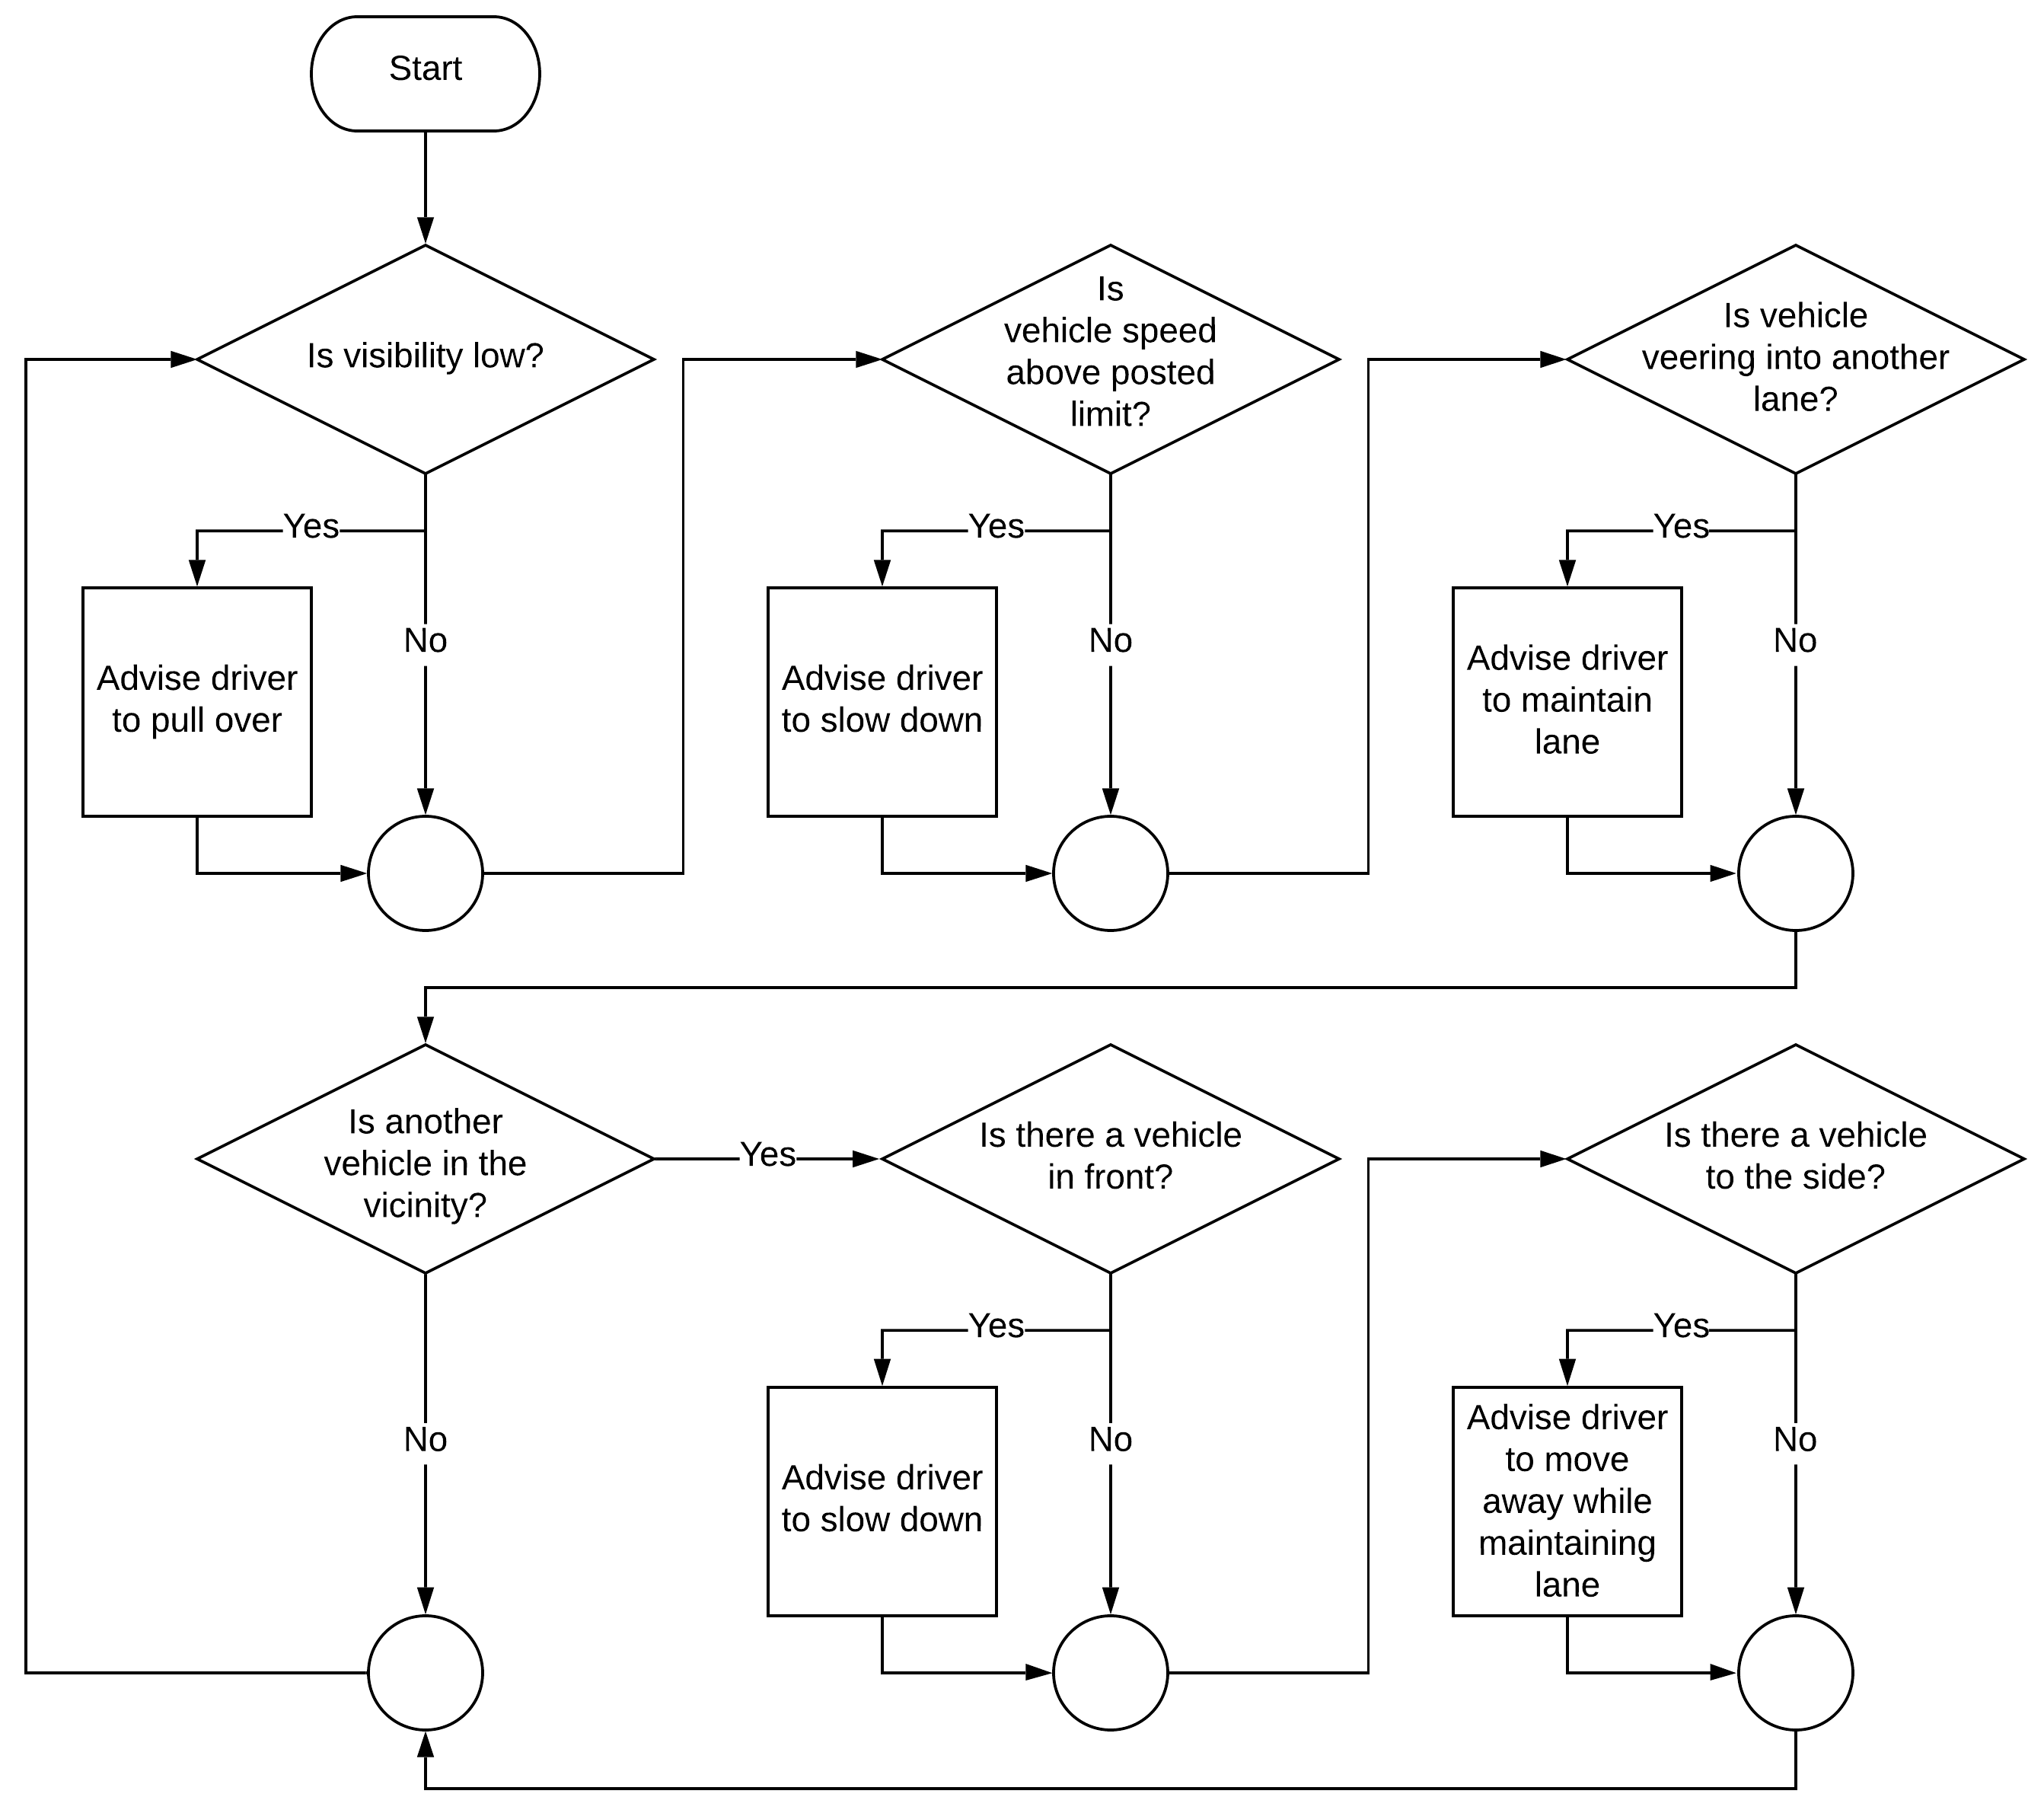
\includegraphics[width=20cm]{workflow.png}}
\end{figure}

\section{Business Rules}
\begin{itemize}
	\item{Cory should be on when the car starts}
	\item{Cory should detect if the driver is going over the speed limit and advise the driver to decelerate}
	\item{Cory should detect if there is a car in front that is too close to the driver and advise the driver to decelerate}
	\item{Cory should detect if the driver is steering into another lane and advise the driver to steer back into their lane}
	\item{Cory should detect if there are cars that are too close to the sides of the car and advise the driver to steer left or right accordingly}
	\item{Cory should detect if visibility is too low and advise the driver to pull over}
\end{itemize}

\section{States and Transitions}
\subsection{Set of States, Input and Output Sets}
\begin{table}[h]
\centering
\begin{tabular}{@{}lll@{}}
\toprule
Abbreviation & Expanded Form & Meaning                                              \\ \midrule
S            & Start         & Cory software is on (Initial state)                  \\
DEC          & Decelerate    & Cory tells the driver to decelerate the car          \\
SL           & Steer Left    & Cory tells the driver to steer left within the lane  \\
SR           & Steer Right   & Cory tells the driver to steer right within the lane \\
PO           & Pull Over     & Cory tells the driver to pull over                   \\ \bottomrule
\end{tabular}
\caption{Set of States}
\label{tab:my-table}
\end{table}

\begin{table}[h]
\centering
\begin{tabular}{@{}ll@{}}
\toprule
Input                       & Output                                         \\ \midrule
AS: Above speed limit       & A: Accelerate message                          \\
FC: Front car too close     & D: Decelerate message                          \\
STL: Steering too far left  & SLL: Steer left while staying in lane message  \\
STR: Steering too far right & SRL: Steer right while staying in lane message \\
LC: Left car too close      & POS: Pull over to side message                 \\
RC: Right car too close     & —: No message                                  \\
VL: Visibility too low      &                                                \\
CNS: Car not stopped        &                                                \\ \bottomrule
\end{tabular}
\caption{Input and Output Sets}
\label{tab:my-table}
\end{table}

\newpage
\subsection{State Transitions}
\subsubsection{Start (S)}
\begin{itemize}
	\item{If car is going over speed limit, go to DEC}
	\item{If there is a car too close in front of the car, go to DEC}
	\item{If the car is steering towards the left lane, go to SR}
	\item{If the car is steering towards the right lane, go to SL}
	\item{If there is a car too close to the left side of the car, go to SR}
	\item{If there is a car too close to the right side of the car, go to SL}
	\item{If visibility is too low, go to PO} 
\end{itemize}

\subsubsection{Decelerate (DEC)}
\begin{itemize}
	\item{If the car is still over the speed limit, stay in DEC}
	\item{If the car in front is still too close, stay in DEC}
	\item{Else, go back to S}
\end{itemize}

\subsubsection{Steer Left (SL)}
\begin{itemize}
	\item{If the car is still steering towards the right, stay in SL}
	\item{If the car on the right is still too close, stay in SL}
	\item{Else, go back to S}
\end{itemize}


\subsubsection{Steer Right (SR)}
\begin{itemize}
	\item{If the car is still steering towards the left, stay in SR}
	\item{If the car on the left is still too close, stay in SR}
	\item{Else, go back to S}
\end{itemize}

\subsubsection{Pull Over (PO)}
\begin{itemize}
	\item{If the car has not pulled over and visibility is still too low, stay in PO}
	\item{Else, go back to S}
\end{itemize}

\newpage
\section{Finite State Machine}
\begin{figure}[h]
	\centerline{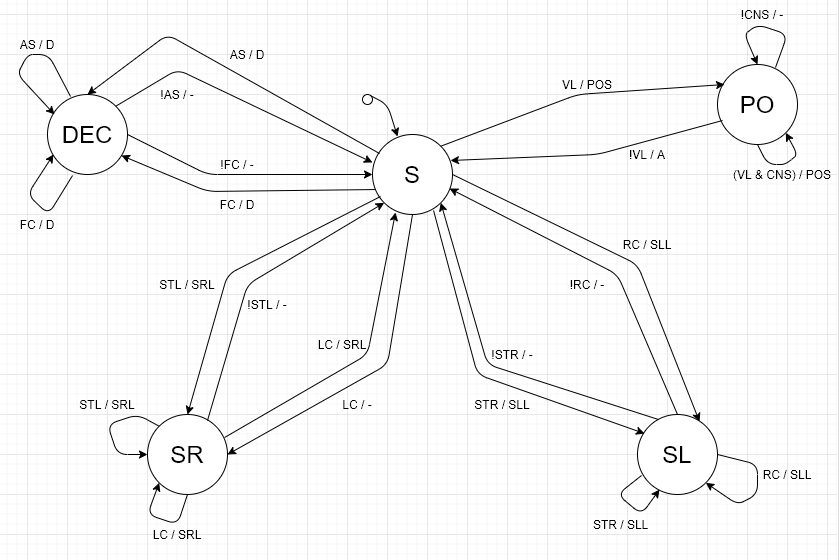
\includegraphics[width=20cm]{fsm.png}}
\end{figure}

\newpage
\section{Test Generation}
\subsection{Transition Tour - Start, Pull Over, Start}
Scenario: Visibility is low.

Sequences:
\begin{itemize}
	\item{$<$S, VL : POS, PO$>$}
	\item{$<$PO, !VL : A, S$>$}
\end{itemize}

\subsection{Transition Tour - Start, Decelerate, Start}
Scenario: Driver is speeding.

Sequences:
\begin{itemize}
	\item{$<$S, AS : D, DEC$>$}
	\item{$<$DEC, !AS :—, S$>$}
\end{itemize}


\end{document}